\documentclass{article}

\title{Podstawy steganografii i steganoanalizy}
\author{Dominik Lau, Sebastian Kutny, Tomasz Lewandowski, Maciej Krzyżanowski}

\usepackage{blindtext}
\usepackage{amsmath}
\usepackage[utf8]{inputenc}
\usepackage[polish]{babel}
\usepackage[T1]{fontenc}
\usepackage{listings}
\usepackage{color}
\usepackage{amssymb}
\usepackage{esvect}
\usepackage{graphicx}
\usepackage{hyperref}
\usepackage{float}


\graphicspath{ {./obrazy/} }

\definecolor{dkgreen}{rgb}{0,0.6,0}
\definecolor{gray}{rgb}{0.5,0.5,0.5}
\definecolor{mauve}{rgb}{0.58,0,0.82}

\lstset{frame=tb,
  language=Python,
  aboveskip=3mm,
  belowskip=3mm,
  showstringspaces=false,
  columns=flexible,
  basicstyle={\small\ttfamily},
  numbers=none,
  numberstyle=\tiny\color{gray},
  keywordstyle=\color{blue},
  commentstyle=\color{dkgreen},
  stringstyle=\color{mauve},
  breaklines=true,
  breakatwhitespace=true,
  tabsize=3
}


\begin{document}

\maketitle

\tableofcontents

\section{Czym jest steganografia? Do czego służy?}
Steganografia polega na ukrywaniu informacji przez ukrywanie komunikacji w innej formie transmisji danych
np. w obrazkach,  plikach dźwiękowych, tekstowych.  Zastosowania steganografii
\begin{itemize}
	\item omijanie cenzury/szpiegostwo
	\item umieszczanie znaków wodnych
	\item ukryta wymiana danych
	\item dodawanie metadanych do plików (np. znaki sterujące)
	\item numery seryjne drukarek (za pomocą małych kropek)
	\item wprowadzanie opóźnień w pakietach sieciowych
	\item zastosowania w VoIP (steganofonia)
	\item zabezpieczanie banknotów (np. EURion constellation)
\end{itemize}
\begin{figure}
	\centering
	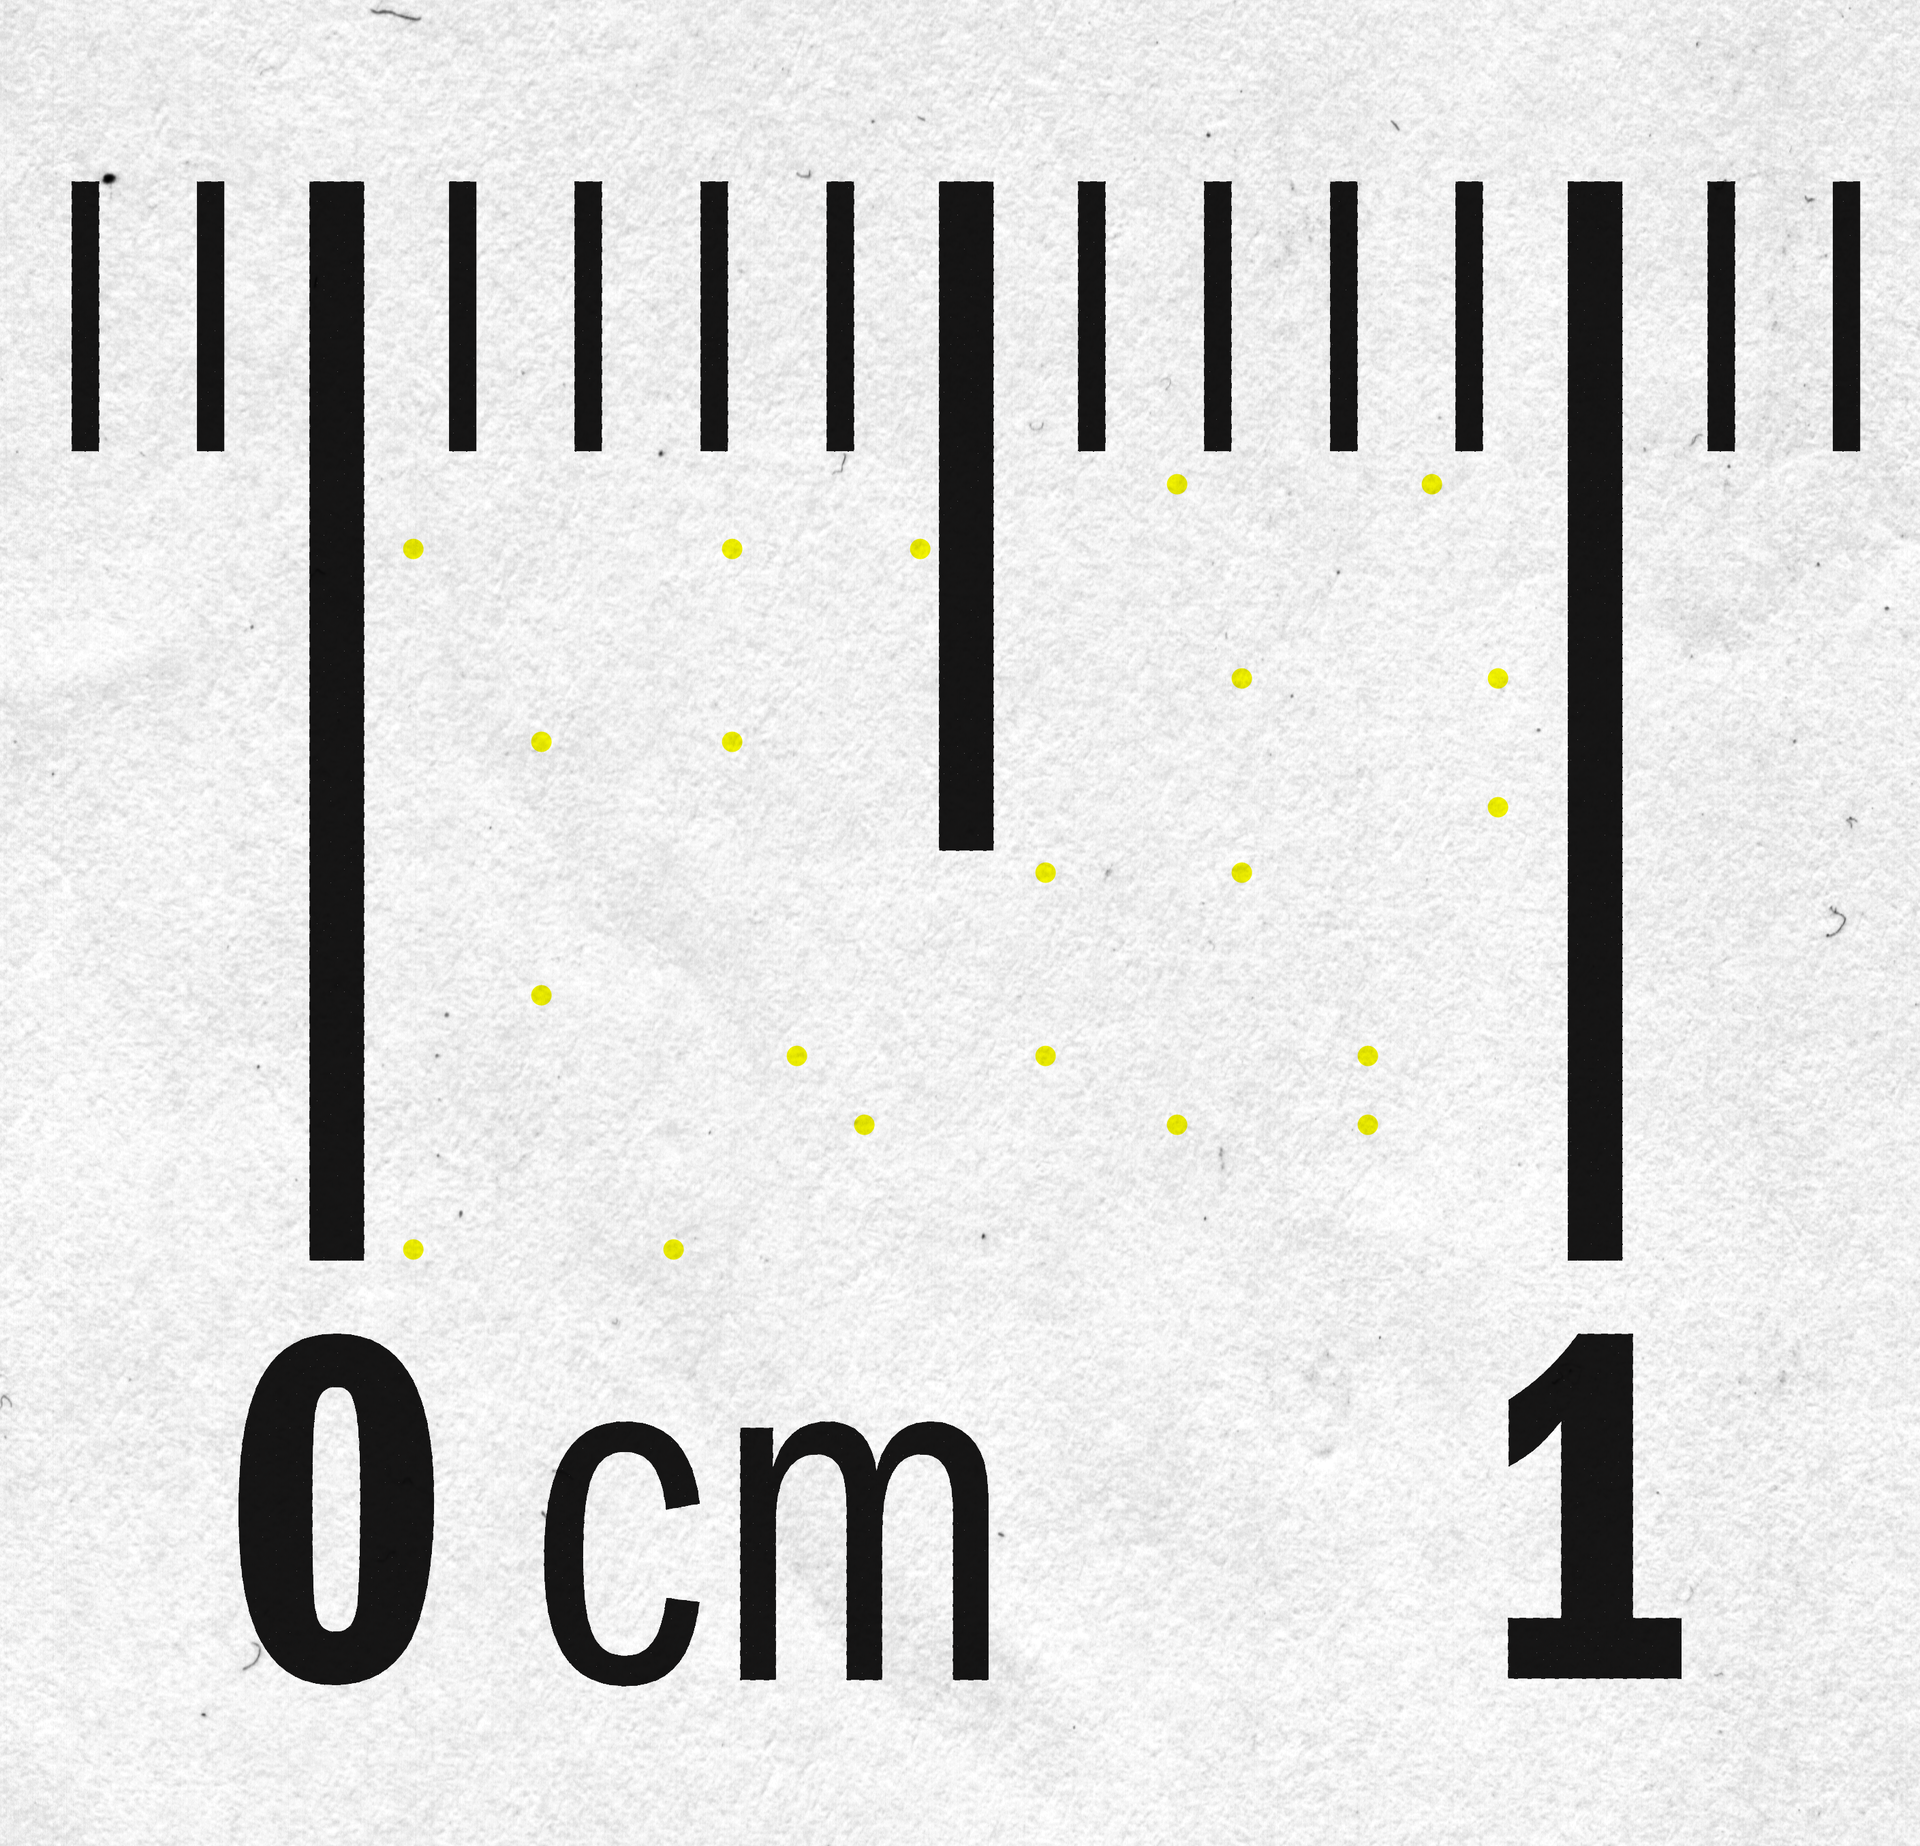
\includegraphics[width=5cm]{stego_drukarkowa}
	\caption{"kropki" zamieszczane przez drukarki}
\end{figure}
Steganografia może zatem realizować następujące funkcje bezpieczeństwa
\begin{itemize}
	\item poufność
	\item autentyczność
	\item niezaprzeczalność
	\item integralność
\end{itemize}
Porównanie kryptografii i steganografii
\begin{center}
\begin{tabular}{c | c  c }
& kryptografia & steganografia \\
\hline
cel & zapewnienie poufności & ukrycie komunikacji \\
obecność klucza & tak & opcjonalna \\
widoczność danych & nie & tak \\
modyfikacja struktury  \\
 przetwarzanych danych & nie & tak
\end{tabular}
\end{center}
\subsection{Słowniczek}
\begin{itemize}
	\item stegosystem - połączenie metod i narzędzi służących do tworzenia ukrytego kanału do przekazywania informacji
	\item wiadomość (payload) - przesyłane dane
	\item kontener/nośnik (carrier) - to wszelkie dane służące do ukrycia tajnej wiadomości
	\item stegokontener - dane i ukryta w nich tajna wiadomość
	\item kanał steganograficzny (stegochannel) - kanał transmisji stegokontenera
	\item klucz (stegokey) - tajny klucz potrzebny do ukrycia stegokontenera
\end{itemize}
\begin{figure}
	\centering
	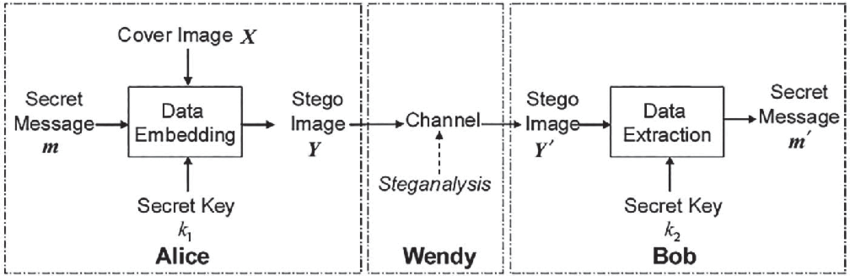
\includegraphics[width=8cm]{model_steganografii}
	\caption{model steganografii}
\end{figure}
\subsection{Podział steganografii}
Ze względu na kontener
\begin{itemize}
	\item w plikach tekstowych
	\item w plikach audio
	\item w obrazach
	\item w ramkach różnych protokołów
	\item w plikach wykonawczych
	\item inne...
\end{itemize}
Ze względu na metodę modyfikacji nośnika
\begin{itemize}
	\item \textbf{metody substytucji} - zamiana nadmiarowych danych nośnika
	\item \textbf{metody transformacyjne} - modyfikacja postaci falowej nośnika
	\item metody statystyczne - modyfikacja właściwości statystycznych nośnika
	\item metody generacji nośnika - ukrywanie informacji podczas tworzenia samego nośnika
	\item metody rozproszonego widma - ukrycie poprzez rozpraszanie danych
	\item metody zniekształceniowe - wprowadzenie zniekształceń do nośnika i pozyskanie informacji poprzez porównanie nośnika oryginalnego i zniekształconego
\end{itemize}
\section{Przykłady rzeczywistych zastosowań steganografii}
\subsection{Historyczne przykłady użycia steganografii}
Pierwsze wzmianki o użyciu technik steganograficznych można odnaleźć u Herodota w V wieku p.n.e.   Opisuje on sposób tajnego przekazu informacji: tyran Histiajos przetrzymywany przez króla perskiego Dariusza postanowił przesłać informację do swego zięcia Arystagorasa z Miletu, tak aby mogła się ona przedostać mimo pilnujących go strażników. Aby tego dokonać na wygolonej głowie swego niewolnika wytatuował przesłanie. Kiedy niewolnikowi odrosły włosy posłał go z oficjalnym, mało istotnym listem. W starożytnym Egipcie i Chinach stosowano atrament sympatyczny, czyli
zapis wiadomości bezbarwną substancją (np. sok z cytryny, który zyskuje barwę przy podgrzaniu). Ponadto już podczas wojny francusko-pruskiej w 1871 a także 2 Wojny Światowej Niemcy wykorzystywali technikę mikrokropek wklejanych
do tekstu maszynopisu. Na mikrokropkach widoczne były zdjęcia wysokiej rozdzielczości.
\begin{figure}[H]
	\centering
	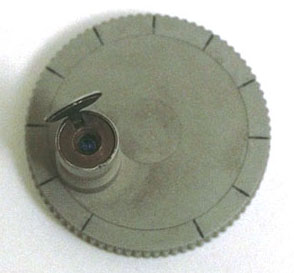
\includegraphics[width=5cm]{mikrokropkowiec}
	\caption{aparat do wykonywania mikrokropek, skala pomniejszenia ok. 1:300}
\end{figure}
\subsection{Eurion}
\begin{figure}[H]
	\centering
	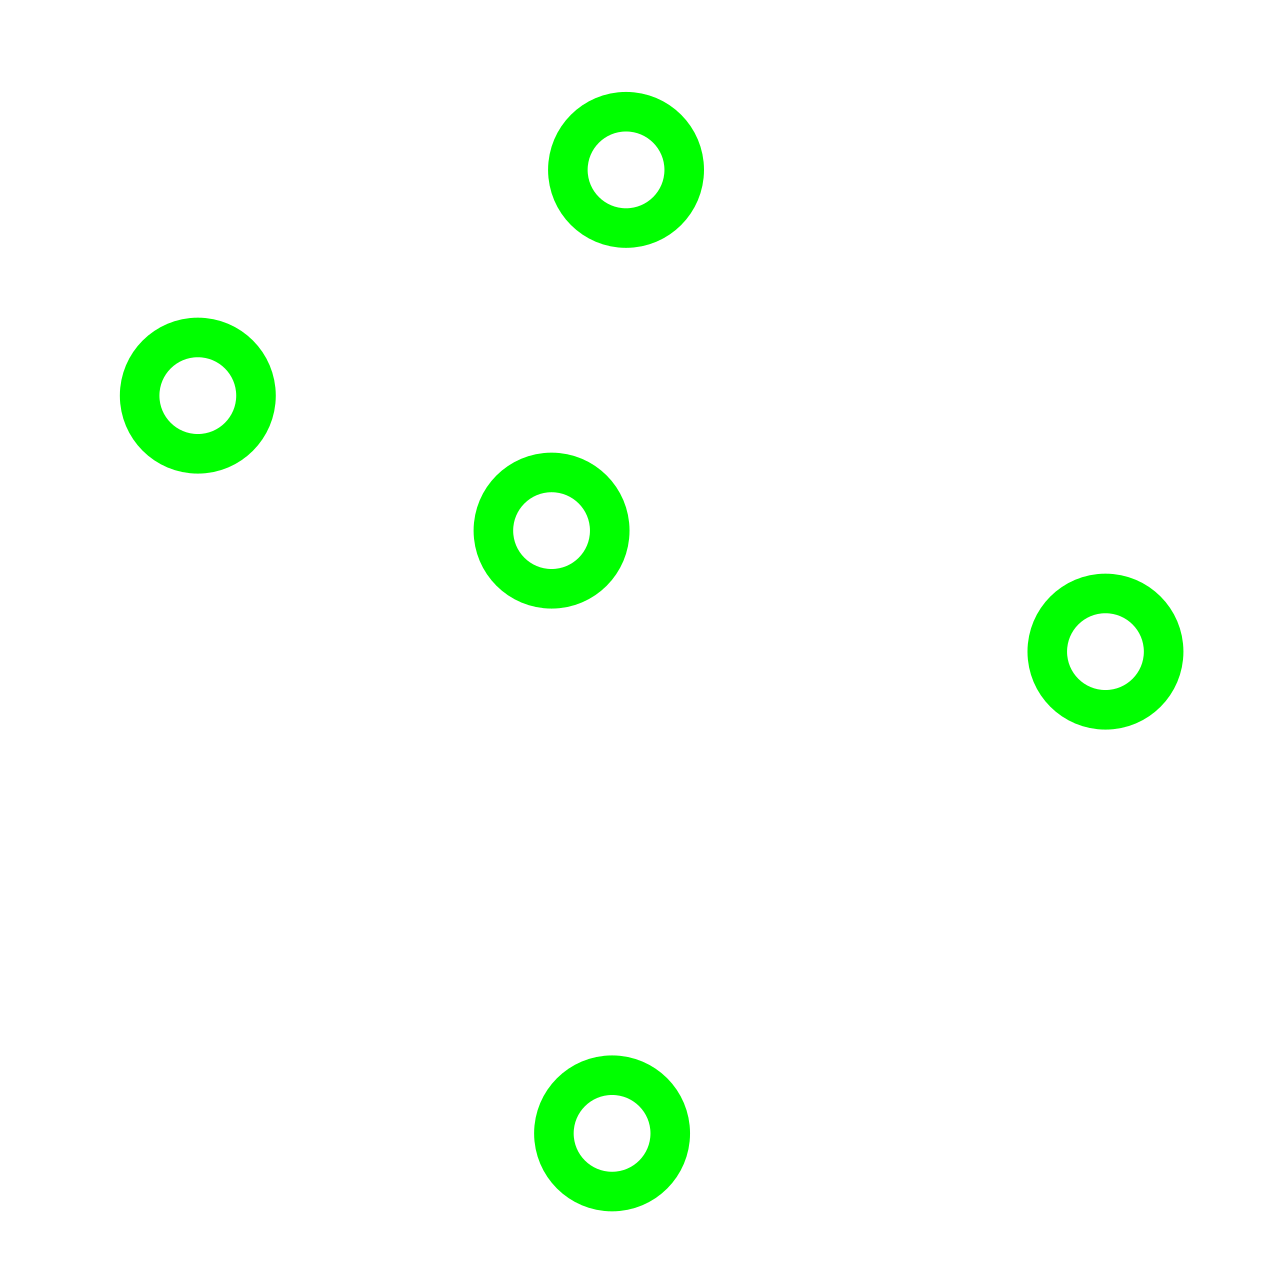
\includegraphics[width=5cm]{eurion}
	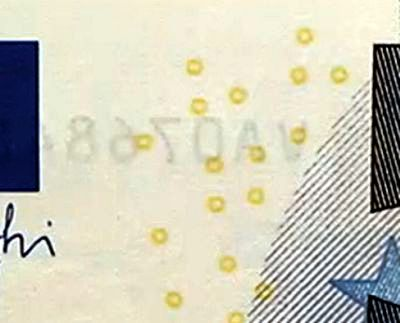
\includegraphics[width=5cm]{euro}
	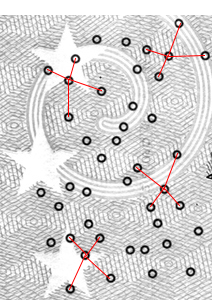
\includegraphics[width=5cm]{close}
	\caption{EURion, przykładowy układ na banknocie euro, dollarze}
\end{figure}
EURion jak i inne podobne zabiegi stanowią metodę przeciwdziałania fałszerstwom. Na banknotach umieszczane
są zbiory kropek o różnych średnicach i względnych pozycjach (te parametry są sekretem). Kropki te tworzą
fingerprint, który jest wykrywany przez oprogramowanie do skanowania (za pomocą metod detekcji wzorca) i
wszelkie próby kopiowania banknotów są blokowane.  
\subsection{Znaki wodne}
Umieszczanie znaków wodnych w plikach ma na celu zamieszczenie informacji o właścicielu praw autorskich.
Wykorzystujemy różnych metod steganografii w celu zapewnienia:
\begin{itemize}
	\item trudności w usunięciu
	\item odporności na transformacje (\textbf{robustness})
	\item niedostrzegalności (\textbf{perceptibility})
	\item przepustowość
\end{itemize} 
z czego najważniejszą cechą jest odporność na transformacje
\begin{figure}[H]
	\centering
	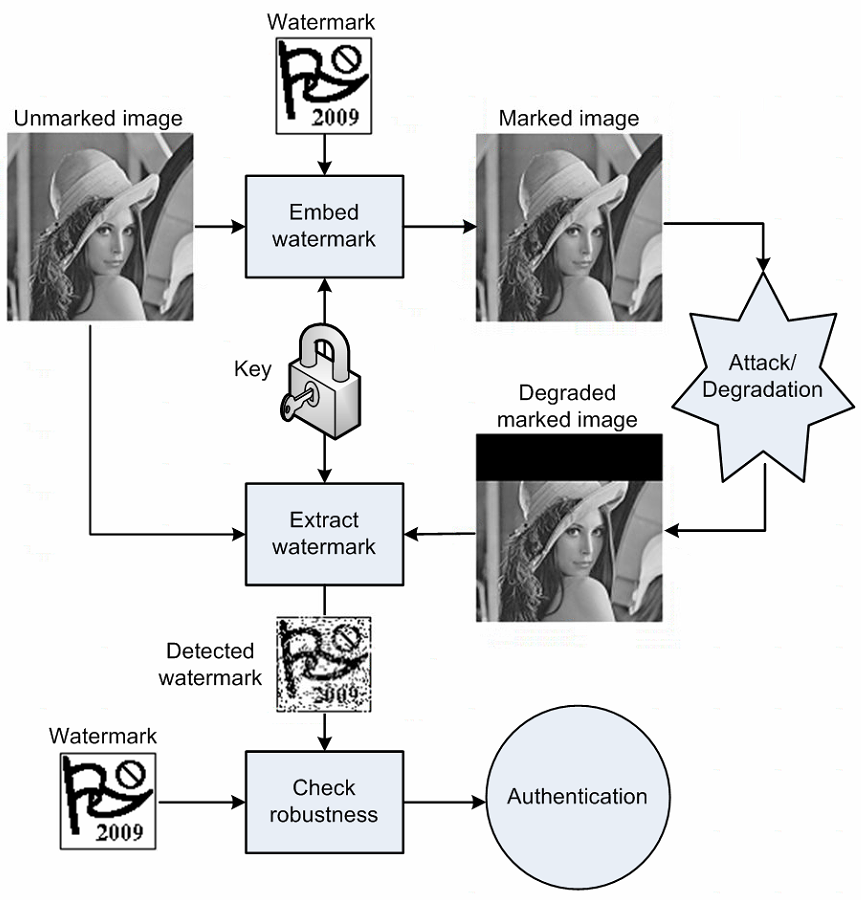
\includegraphics[width=6cm]{watermark}
	\caption{schemat zamieszczania znaku wodnego}
	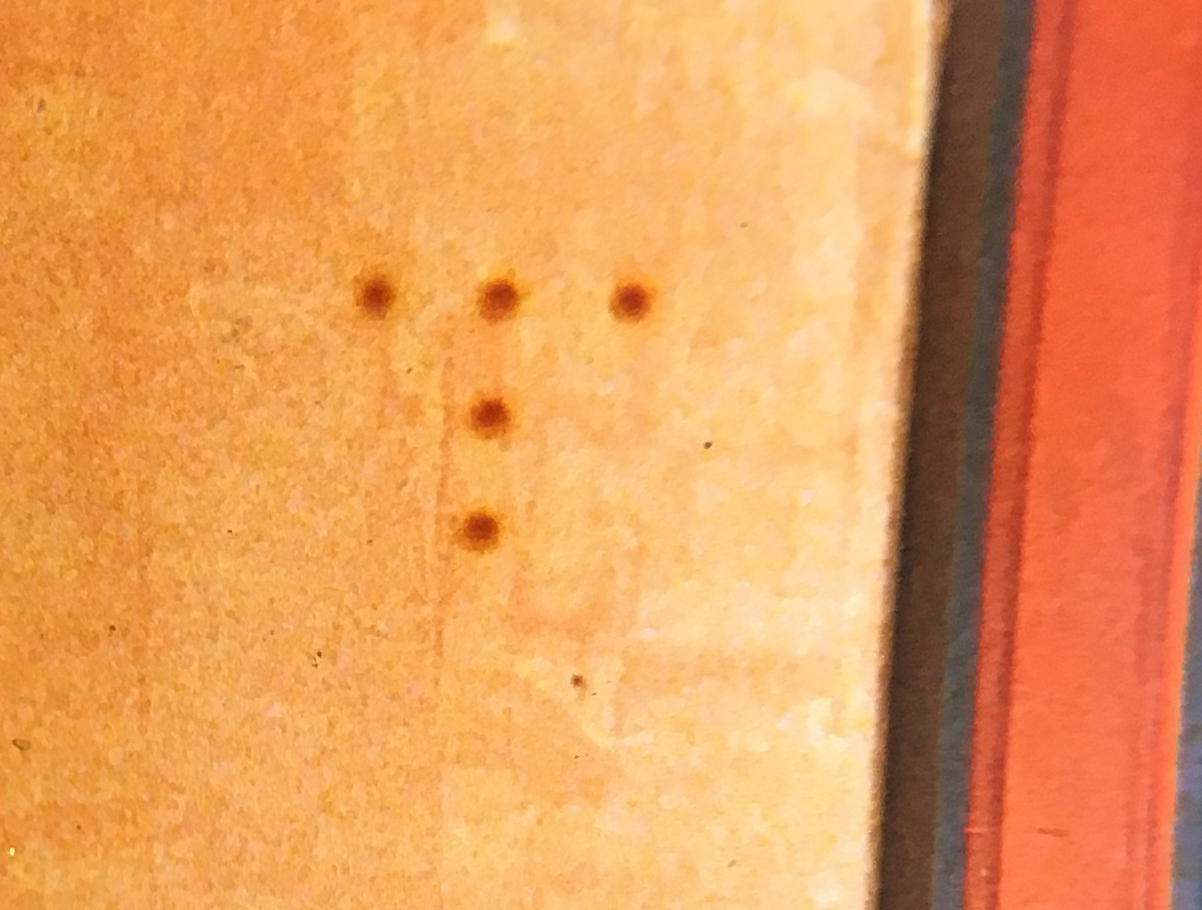
\includegraphics[width=4cm]{cap}
	\caption{CAP(Coded Anti Piracy) - przykład znaku wodnego zamieszczanego w filmach do identyfikacji źródła nielegalnych kopii}
\end{figure}
\section{Przegląd technik steganografii}
\subsection{Modyfikacja LSB obrazu}
Jest to klasyczny algorytm steganografii, którego główną wadą jest łatwość w wykryciu/zniszczeniu wiadomości
(np. przez wyzerowanie najmłodszych bitów). Przed niechcianym odczytem wiadomości możemy zapobiec 
poprzez zastosowanie kryptografii. Zasada działania algorytmu jest prosta:
\begin{enumerate}
	\item wybierz, w którym kanale zapisać bity wiadomości (r,g,b, a, może obraz czarnobiały?)
	\item zastąp stare wartości najmłodszych bitów określonego kanału obrazu kolejnymi bitami wiadomości
\end{enumerate}
Analogiczna metoda jest możliwa na plikach dźwiękowych, tylko tam zmieniamy LSB próbek.
\subsection{Steganografia gamma - gamma trick}
Wiele programów nie implementuje korekcji gamma (czyli kodowania luminancji obrazu za pomocą nieliniowej charakterystyki $I' = AI^{\gamma}$.


\subsection{Ukrywanie obrazów w spektrogramach}
\begin{figure}[H]
	\centering
	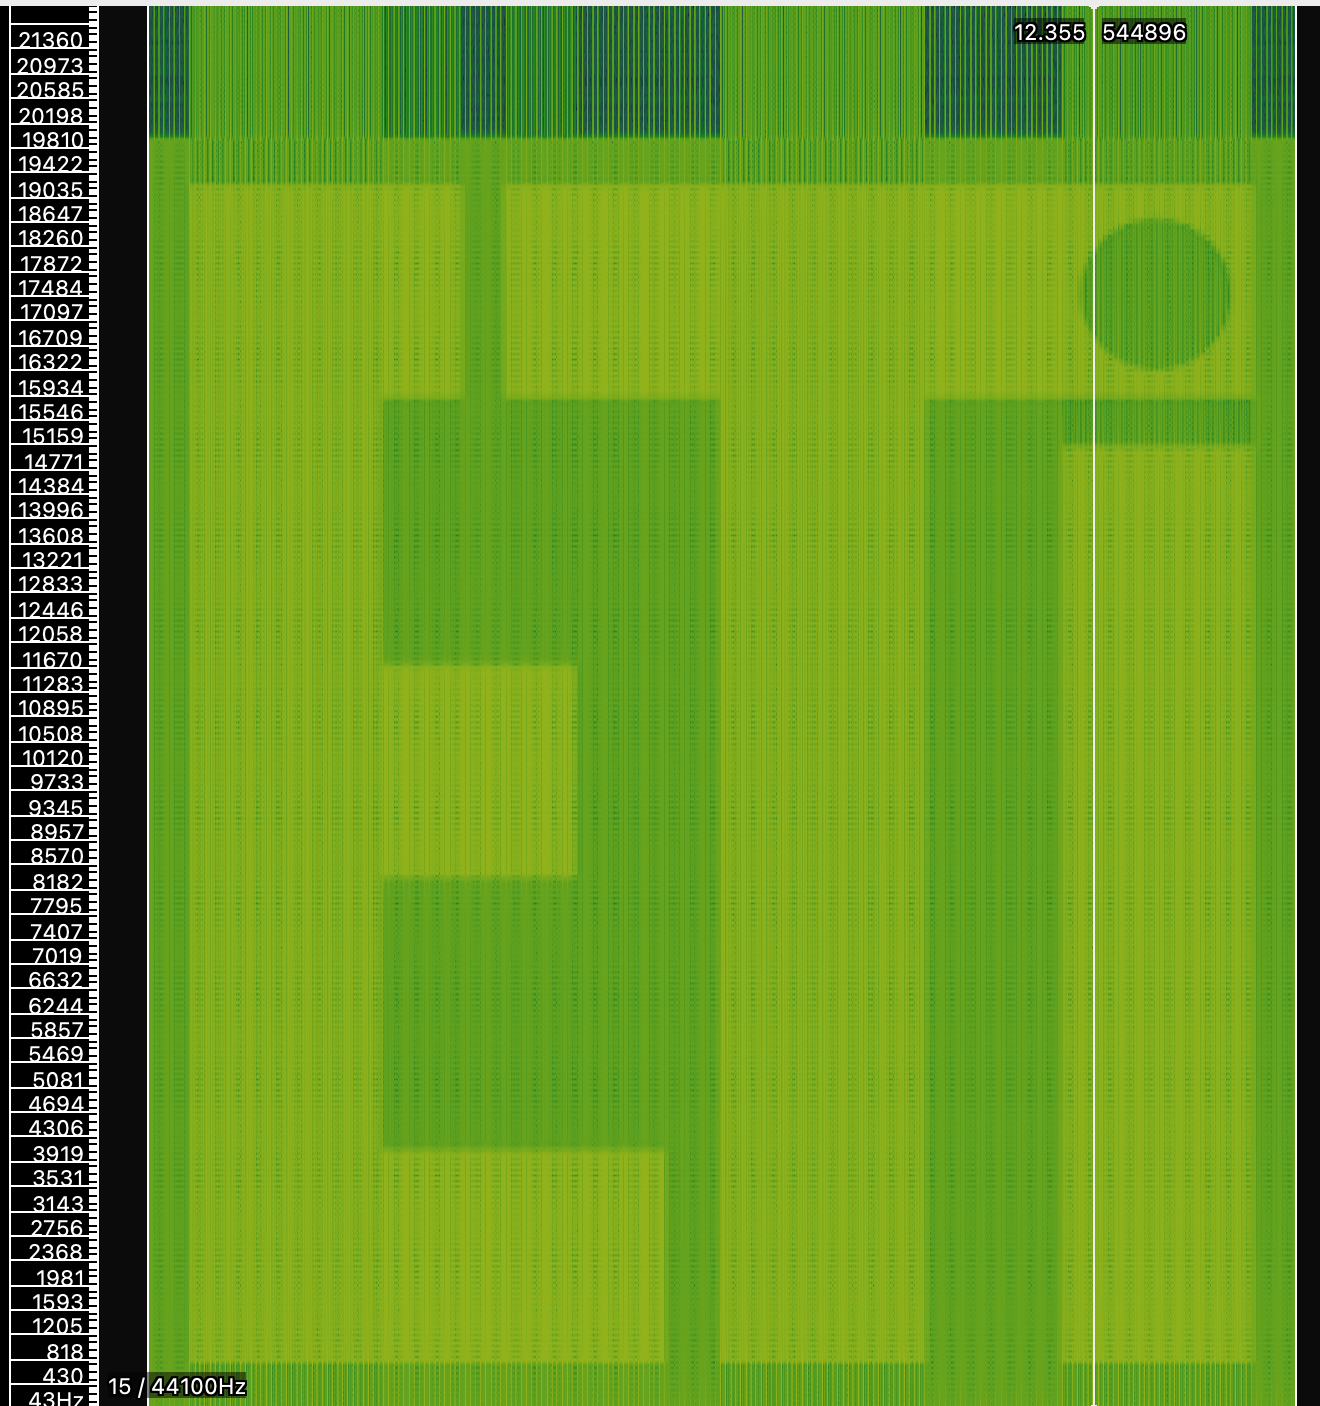
\includegraphics[width=5cm]{samobraz}
	\caption{Obraz zamieniony na dźwięk, bez żadnego "ukrywającego" pliku dźwiękowego, dźwięk
	ten jest odbierany jako szum}
\end{figure}
Inną z technik jest ukrywanie danych w określonych częstotliwościach pliku dźwiękowego.
Jak to działa? Zaczynamy od konwersji obrazu na odcienie szarości.
Następnie korzystamy ze wzoru (IDFT - inverse discrete fourier transform)
\begin{gather*}
	x = \Sigma_{y=0}^{H-1}I[x,y]sin(\frac{2\pi f i}{S})
\end{gather*}
gdzie: \\ 
$H$ to wysokość obrazu, \\
$x$ to próbka odpowiadająca $x$-tej kolumnie obrazu,\\
$I[x,y]$ to jasność piksela o współrzędnych $x,y$, \\
$S$ to częstotliwość próbkowania, \\
$i$ to numer próbki w bloku (odwrotna transformacja Fouriera operuje na blokach stałego rozmiaru,
które łączy w wartość wielomianu w punkcie $x$) \\
rozmiar bloku definiuje szerokość umieszczanego obrazu (w sensie ilości próbek) 
\begin{gather*}
 f = y * \frac{f_{max} - f_{min}}/H + f_{min} 
\end{gather*}
 $f_{min}$ to częstotliwość, od której zaczyna
się dolna krawędź obrazu, $f_{max}$ to górna krawędź (np. $f_{min} = 20$ Hz, $f_{max} = 20$ kHz).
Chcąc dodać ukryty sygnał do istniejącego pliku dźwiękowego dodajemy sygnały
\begin{gather*}
I' = I + \beta x
\end{gather*}
$\beta$ to współczynnik tłumienia mający na celu ukrycie "brzęczenia" ukrytego obrazu
\begin{figure}[H]
	\centering
	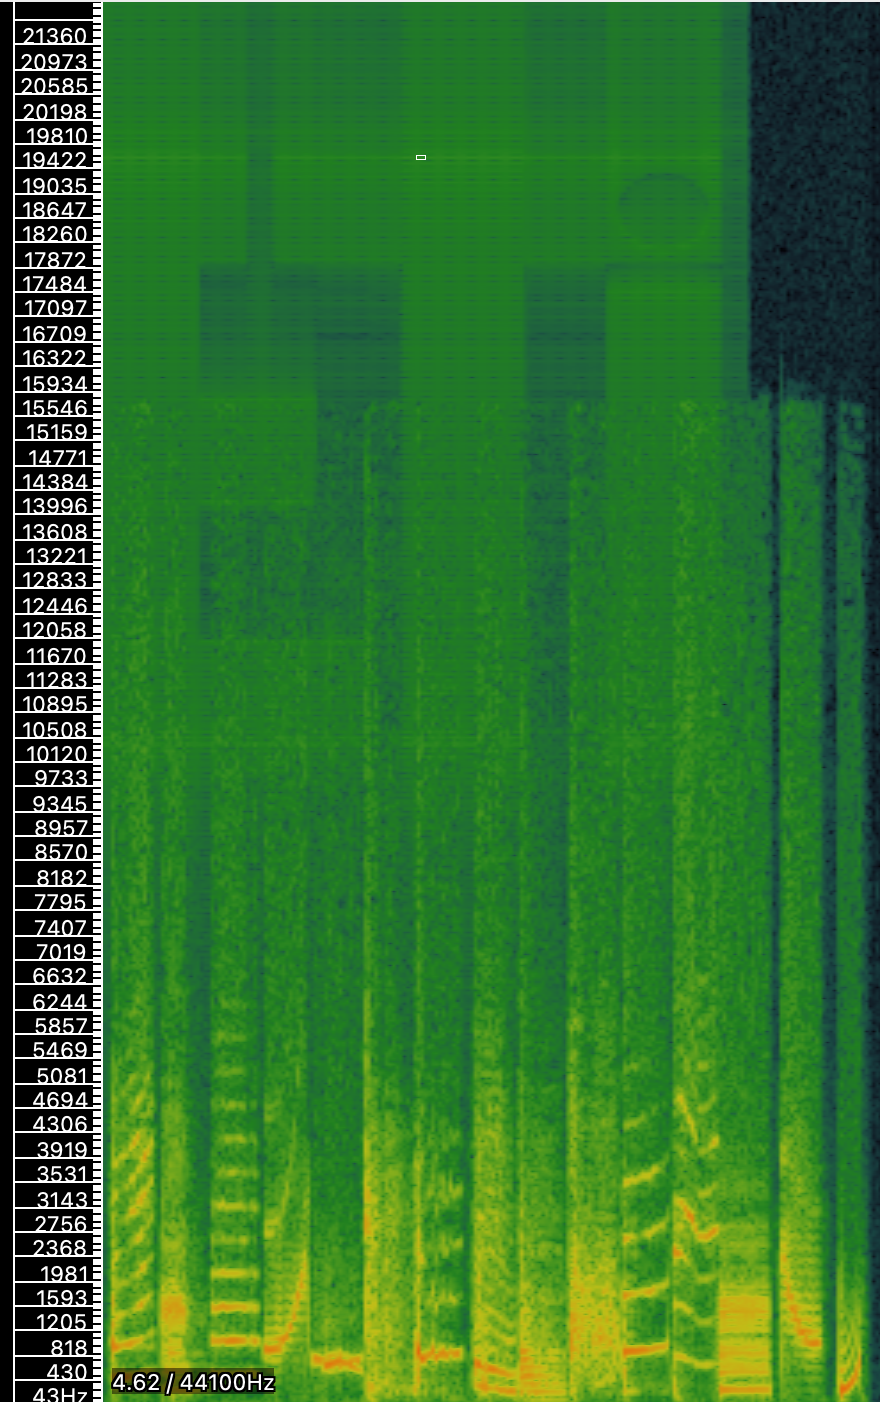
\includegraphics[width=4cm]{gorszajakosc_spektro}
	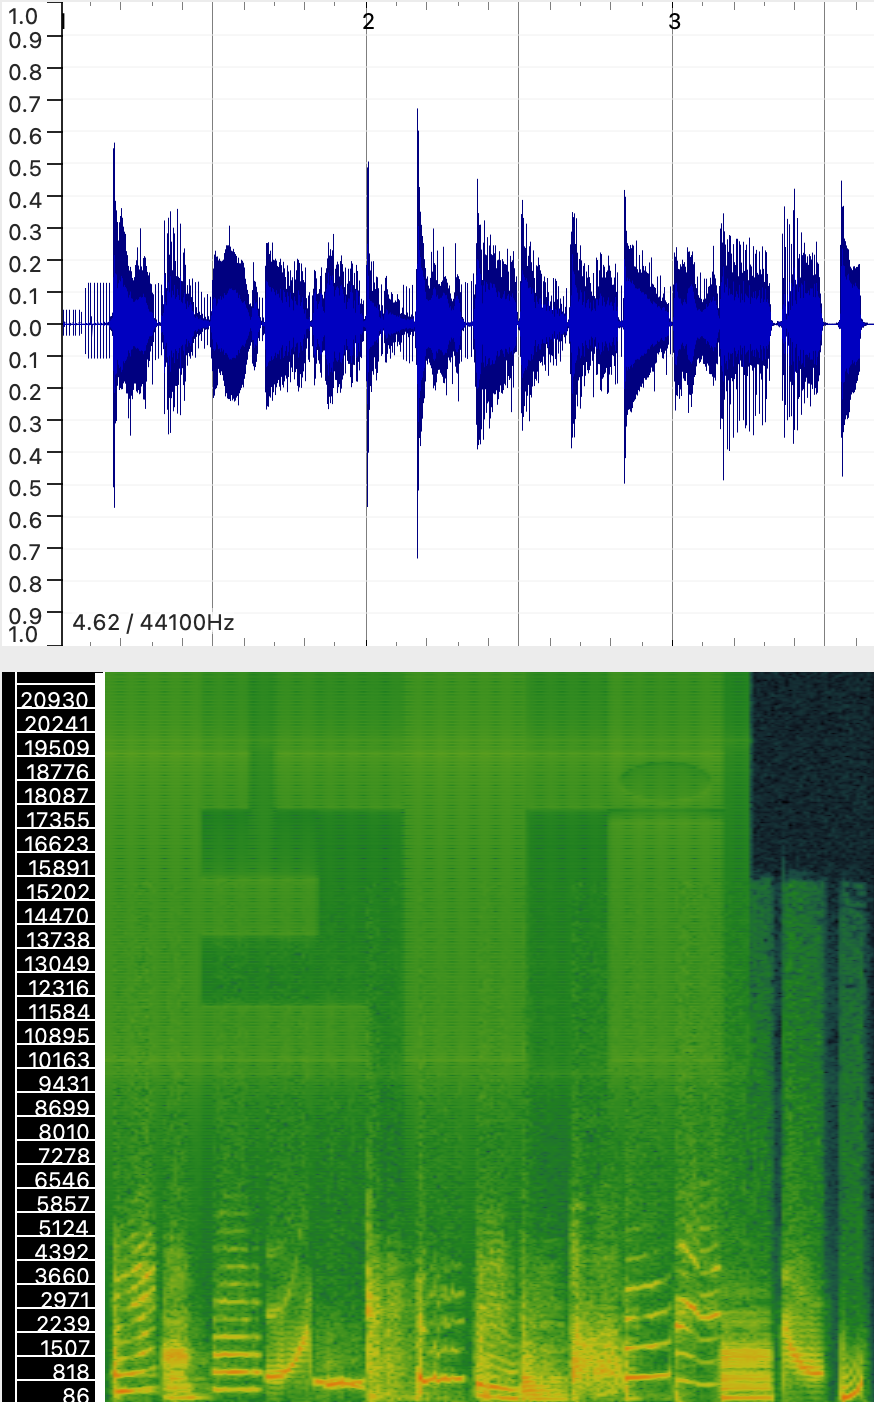
\includegraphics[width=4cm]{szumy_spektro}
	\caption{Z lewej: przytłumiony sygnał obrazu umieszczony w spektrogramie istniejącego pliku dźwiękowego, z prawej: ilustracja szumów przy braku tłumienia obrazu - szum tworzy widoczne gołym okiem wąsy}
\end{figure}
\subsection{Ukrywanie archiwów w obrazach}
Kolejny bardzo prosty sposób na ukrycie danych w obrazach polega na sklejeniu dwóch plików ze sobą, uzyskując tym samym plik polyglot.  Wymaga to jednak, żeby formaty akceptowały "śmieci" przed nagłówkiem.  Przykładami takich
formatów są pdf, rar, zip.
Metodę tą można łatwo wykryć na przykład za pomocą strings/binwalk. \\\\
Zapisywanie:
\begin{lstlisting}[language=bash]
  $ cat microprocessors.jpg JAVA_slajdy.pdf > image.jpg
\end{lstlisting}
W ten sposób ukrywać możemy zwykłe pliki tekstowe
\begin{lstlisting}[language=bash]
  $ cat microprocessors.jpg haslo.txt > image.jpg
\end{lstlisting}
wówczas 
\begin{lstlisting}[language=bash]
 $ strings image.jpg
	...
 	ri]P
	:9w;
	!`{?
	haslo
\end{lstlisting}
\begin{figure}[H]
	\centering
	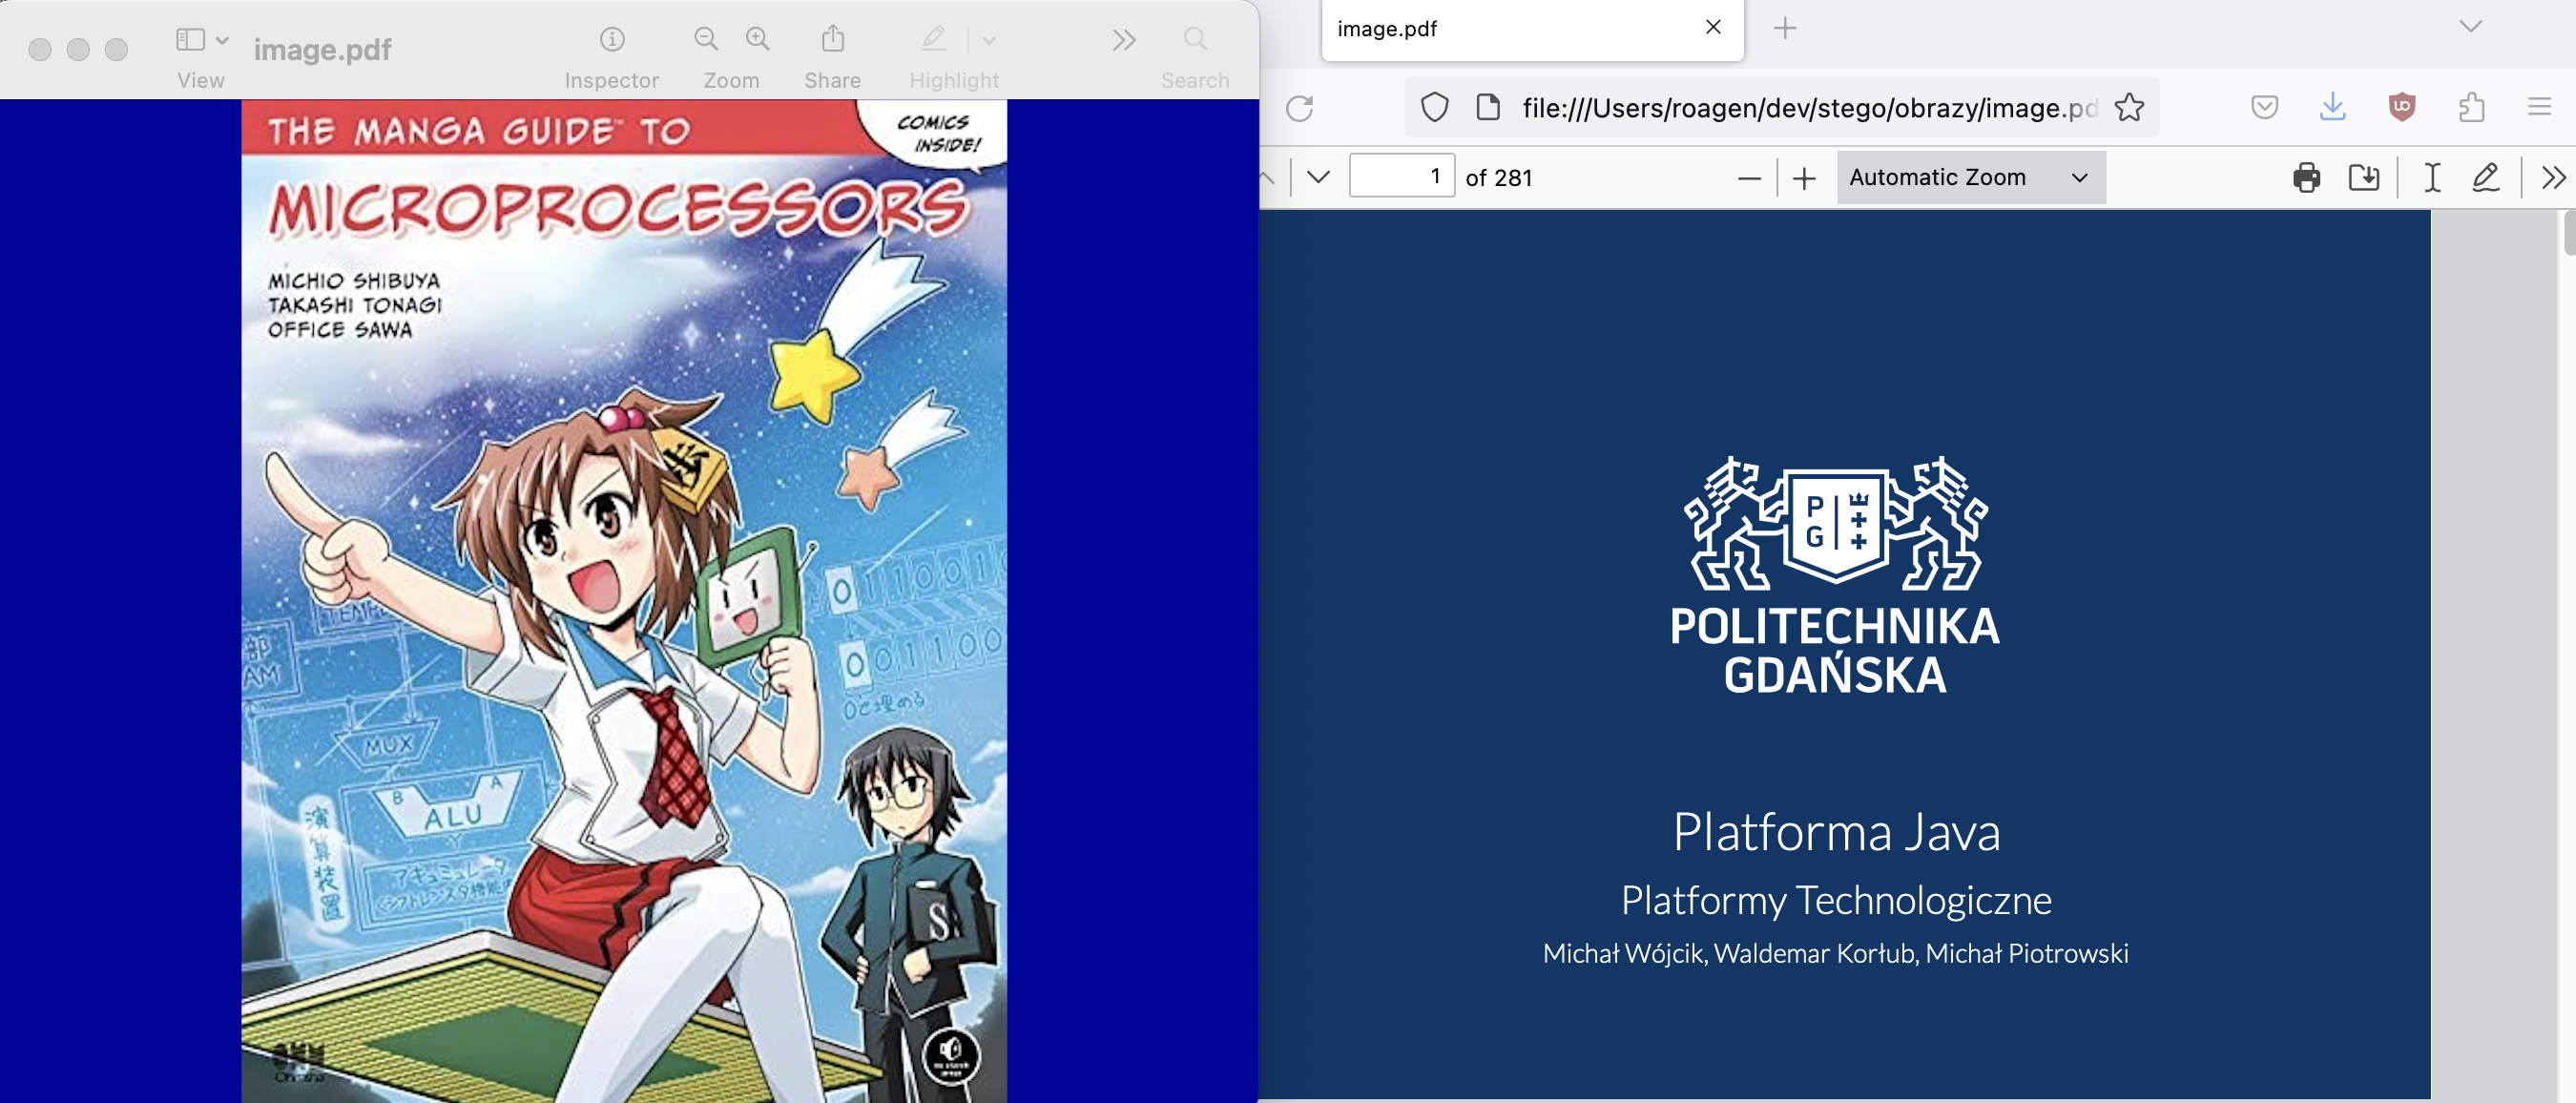
\includegraphics[width=8cm]{sklejanie}
	\caption{Przykład pliku "poligloty", który może być jednocześnie interpretowany jako .jpg i .pdf}
\end{figure}
Szczególnym przypadkiem złączonych plików są pliki \textbf{GIFAR} - gif + jar.  Przy nieodpowiednio zabezpieczonej stronie umożliwiającej umieszczanie gifów atakujący może uruchomić 
kod z pliku jar będącego częścią zamieszczonego gifa.  Jary podobnie jak wszystkie formaty bazujące na formacie zip umożliwiają umieszczanie dodatkowych bajtów przed nagłówkiem.

\subsection{Homoglify - Twitter Steganography}
Homoglify to znaki, których kształty mogą być interpretowane na różne sposoby.  Chcąc przy ich użyciu ukryć wiadomość musimy:
\begin{enumerate}
	\item zdefiniować alfabet wiadomości 
	\begin{itemize}
		\item ile bitów na znak? np.  6
		\item jak wygląda alfabet np.   \_abcdefghijklmnopqrstuvwxyz123456789
		\item dla powyższego alfabetu znak a będzie miał kod 000001 a np.  l 001100
	\end{itemize}
	\item ustalić tekst wiadomości, która będzie kontenerem
	\item ustalić tekst ukrytej wiadomości i przekodować go na alfabet
	\item dla każdego znaku kontenera
	\begin{enumerate}
		\item sprawdzamy ile ma homoglifów $h$
		\item liczbę różnych homoglifów danego znaku możemy zakodować na $ceil(log_2 h) = b$ bitach
		\item bierzemy $b$ bitów ukrywanej wiadomości i na ich podstawie wybieramy, który z homoglifów zapiszemy do tekstu wyjściowego
		\item czyli na przykład, jeżeli pierwsza litera kontenera to A, które ma 4 homoglify, to bierzemy 2 bity wiadomości, jeżeli jest to 00 to znaku nie zmieniamy, 01 - wybieramy pierwszy homoglif itd...
	\end{enumerate}
\end{enumerate}
Żeby zdekodować wiadomość musimy znać alfabet i ilość bitów na znak.
\begin{figure}[H]
	\centering
	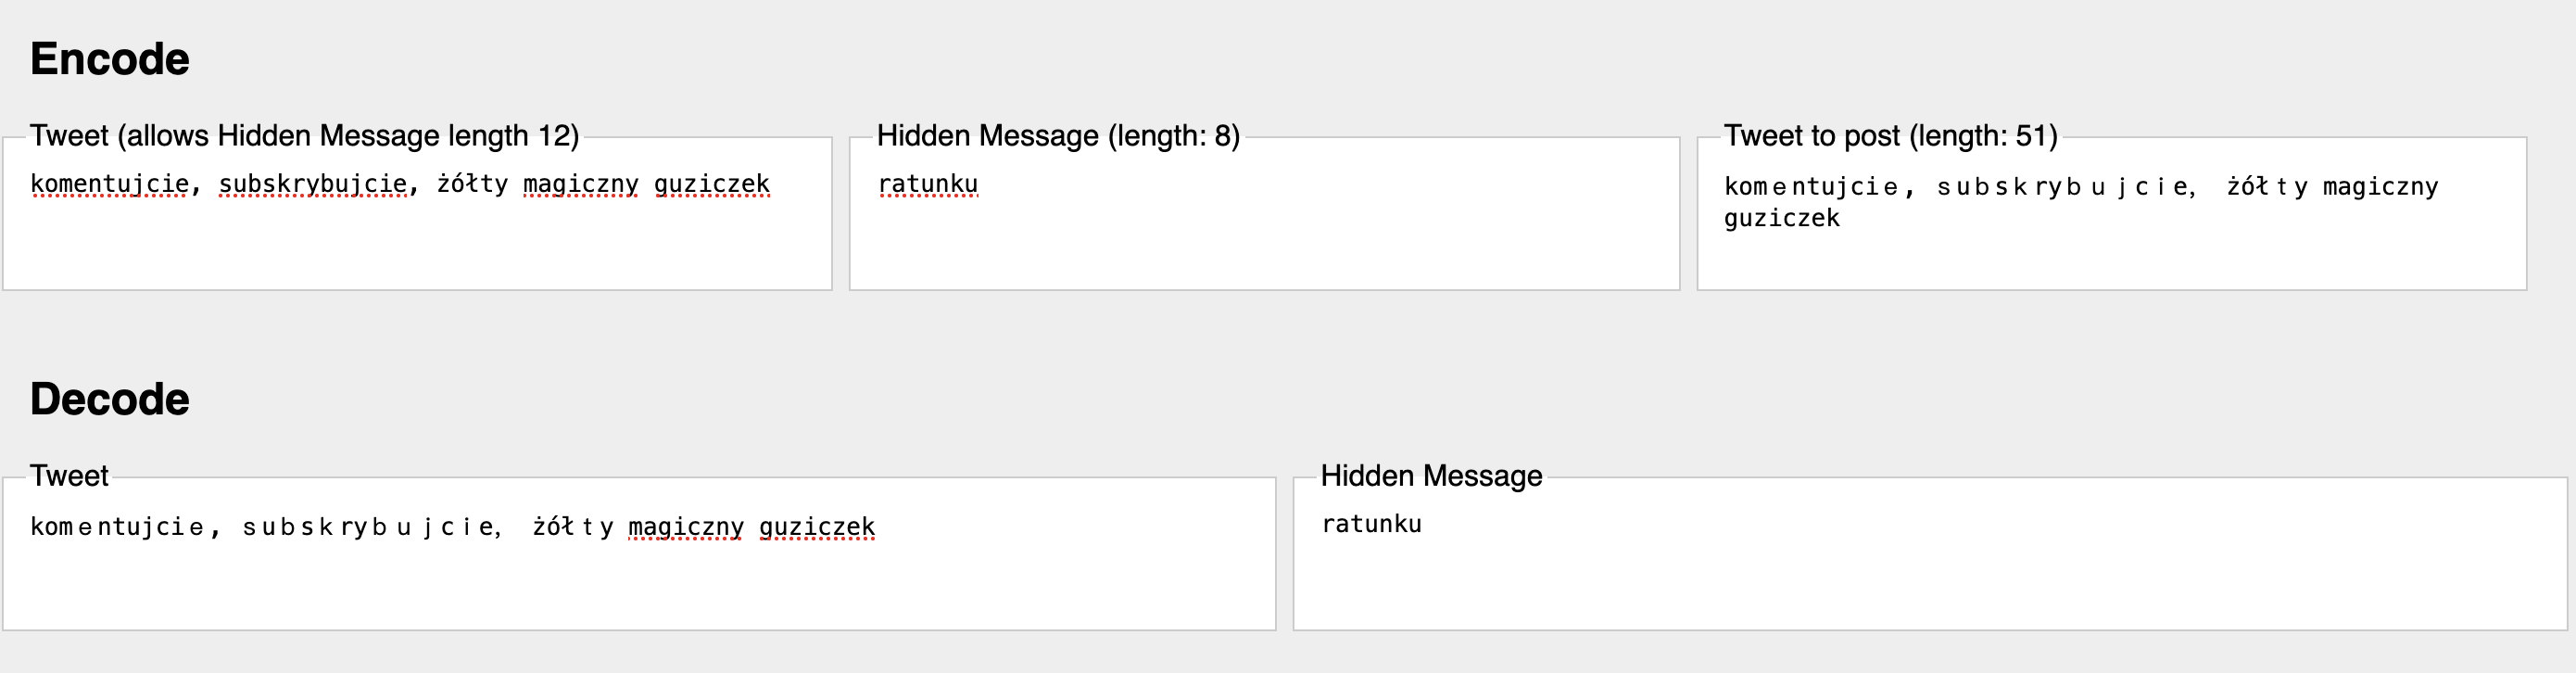
\includegraphics[width=12cm]{homoglify}
	\caption{przykład wiadomości zakodowanej za pomocą Twitter Steganography}
\end{figure}

\subsection{Chaffing i winnowing}
Chaffing i winnowing to metoda z pogranicza kryptografii jak i steganografii. Technikę tą wymyślił Ron Rivest. Załóżmy, że Alicja chce wysłać wiadomość do Bogdana
oraz wymienili między sobą klucz, który będą wykorzystywali w algorytmie MAC. Ponadto pakiety będą wysyłane bit po bicie, bity będą ponumerowane (żeby zachować ich kolejność).
\begin{enumerate}
	\item Alicja wysyła pakiety wiadomości razem z tagiem MAC tych wiadomości
	\item między pakietami losowo wysyła również zanegowane wartości bitów z losowymi wartościami tagu MAC (chaffing)
	\item Bogdan odbiera pakiety i rozważa tylko te, dla których zgadzia się MAC (winnowing)
\end{enumerate}
Metoda ta gwarantuje
\begin{enumerate}
	\item poufność, podsłuchujący nie wie, który pakiet ma poprawny MAC
	\item autentyczność, ponieważ poprawne pakiety są zabezpieczone za pomocą MAC
\end{enumerate}
\begin{figure}[H]
	\centering
	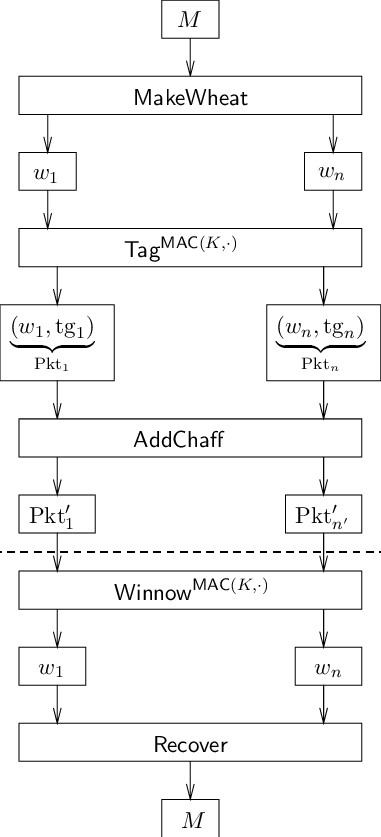
\includegraphics[width=3cm]{chaffingwinnowing}
	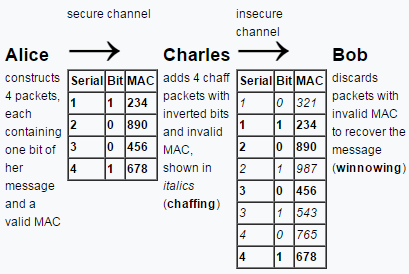
\includegraphics[width=8cm]{chaffingwinnowing2}
	\caption{schemat działania metody i przykład}
\end{figure}


\section{Steganoanaliza}
Steganoanaliza (Steganalysis) jest tym samym dla steganografii, czym kryptoanaliza dla kryptografii - sztuką detekcji ukrytych wiadomości.
Metody steganoanalityczne opierają się głównie na analizie parametrów statystycznych pliku. Przykładowe techniki
\begin{itemize}
	\item analiza widma sygnału (przykładowo przeszukiwanie wysokich częstotliwości)
	\item niespójności w kompresji (np. "edge ringing" w kompresji JPEG)
	\item wykorzystywanie oryginalnego nośnika, jeżeli jest dostępny 
	\item szukanie nietypowych wzorców 
	\item użycie metod uczenia maszynowego
\end{itemize}
\begin{figure}[H]
	\centering
	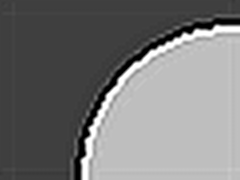
\includegraphics[width=4cm]{edge_ringing}
	
\includegraphics[width=4cm]{noringing}
	\caption{obraz z "edge ringing" i bez - jest to przewidywalne zniekształcenie; proste algorytmy steganografii mogą mieć problem z dobrym 
	odwzorowaniem artefaktów o wysokim prawdopodobieństwie wystąpienia}
\end{figure}
\subsection{Zadania steganoanalizy}
\begin{itemize}
	\item detekcja instnienia kanału steganograficznego (steganoanaliza pasywna)
	\item zniszczenie wiadomości w stegokontenerze
	\item ekstrakcja wiadomości ze stegokontenera
\end{itemize}
\subsection{Problemy steganoanalizy}
\begin{itemize}
	\item wiele szyfrów ma taką właściwość, że produkuje szyfrogramy przypominające szum biały (o kompletnie płaskim widmie),
	\item barrage noise - bombardowanie stegokontenerami z losowymi/bezwartościowymi informacjami
\end{itemize}
\subsection{Steganoanaliza LSB}
Prosta metoda wykrycia, czy obraz zawiera zakodowaną wiadomość
\begin{enumerate}
	\item dzielimy piksele na bloki
	\item dla każdego bloku liczymy wartość średnią LSB
\end{enumerate}
Jeżeli w obrazie ukryto \textbf{zaszyfrowaną} wiadomość, to niektóre regiony bloków
powinny mieć średnią $\approx 0.5$ (ze względu na losowy charakter szyfrów). Możliwe są
oczywiście false positives, gdy piksele w niezmodyfikowanym obrazie mają taką charakterystykę.
\section{Narzędzia steganoanalityczne}
\subsection{strings}
strings to linuxowa komenta wypisująca łańcuchy znaków z danego pliku. Dzięki temu możemy pozyskać informacje 
o metadanych ukrytych np. w plikach wykonawczych
\begin{figure}[H]
	\centering
	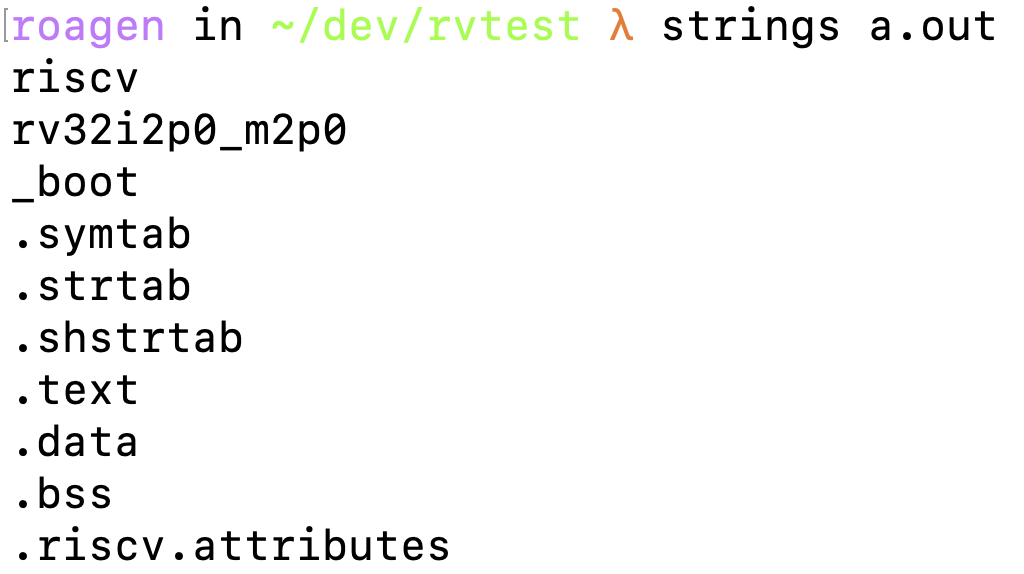
\includegraphics[width=8cm]{strings_example}
	\caption{przykład użycia strings na pliku wykonawczym w architekturze rv32}
\end{figure}
\subsection{binwalk}
jest to program do znajdowania istniejących nagłówków plików w innym pliku, program umożliwia także analizę entropii pliku
\begin{figure}[H]
	\centering
	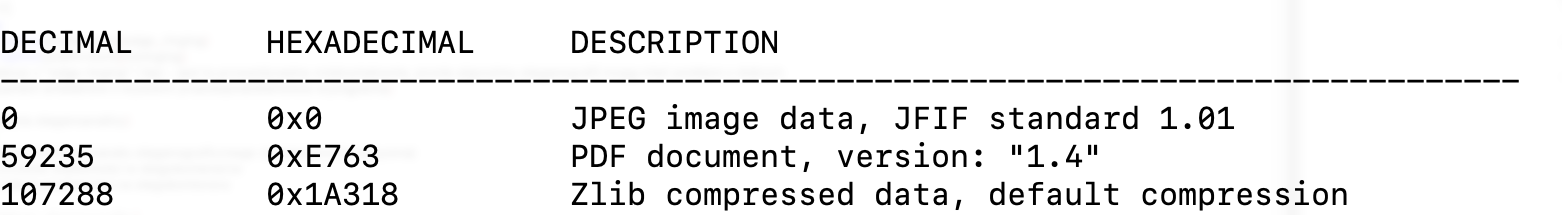
\includegraphics[width=8cm]{binwalk}
	\caption{przykład użycia binwalk na pliku poliglocie jpg + pdf}
\end{figure}
\subsection{StegExpose}
StegExpose to narzędzie do wykrywania steganografii LSB bazujące na metodzie RS,  która jest podobna
do wcześniej omówionej prostej steganoanalizy LSB, z wykorzystaniem teorii grup.
\begin{figure}[H]
	\centering
	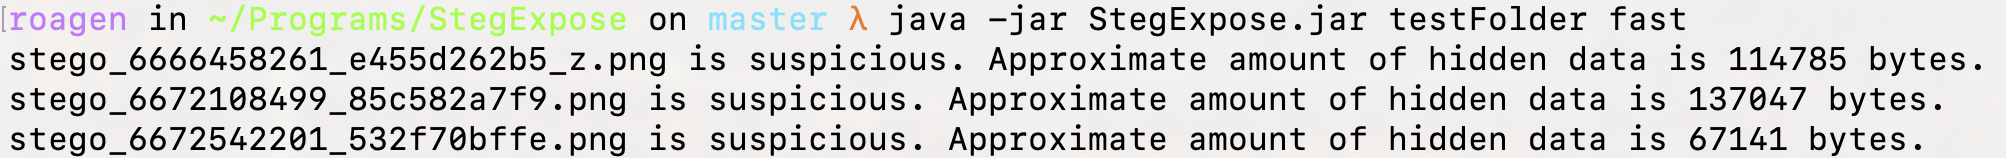
\includegraphics[width=8cm]{stegexpose}
	\caption{przykład użycia StegExpose}
\end{figure}
\subsection{Sonic Visualizer}
Sonic Visualizer to program do wizualizacji plików dźwiękowych, który może być użyteczny do znajdowania
podejrzanych szumów itp.
\begin{figure}[H]
	\centering
	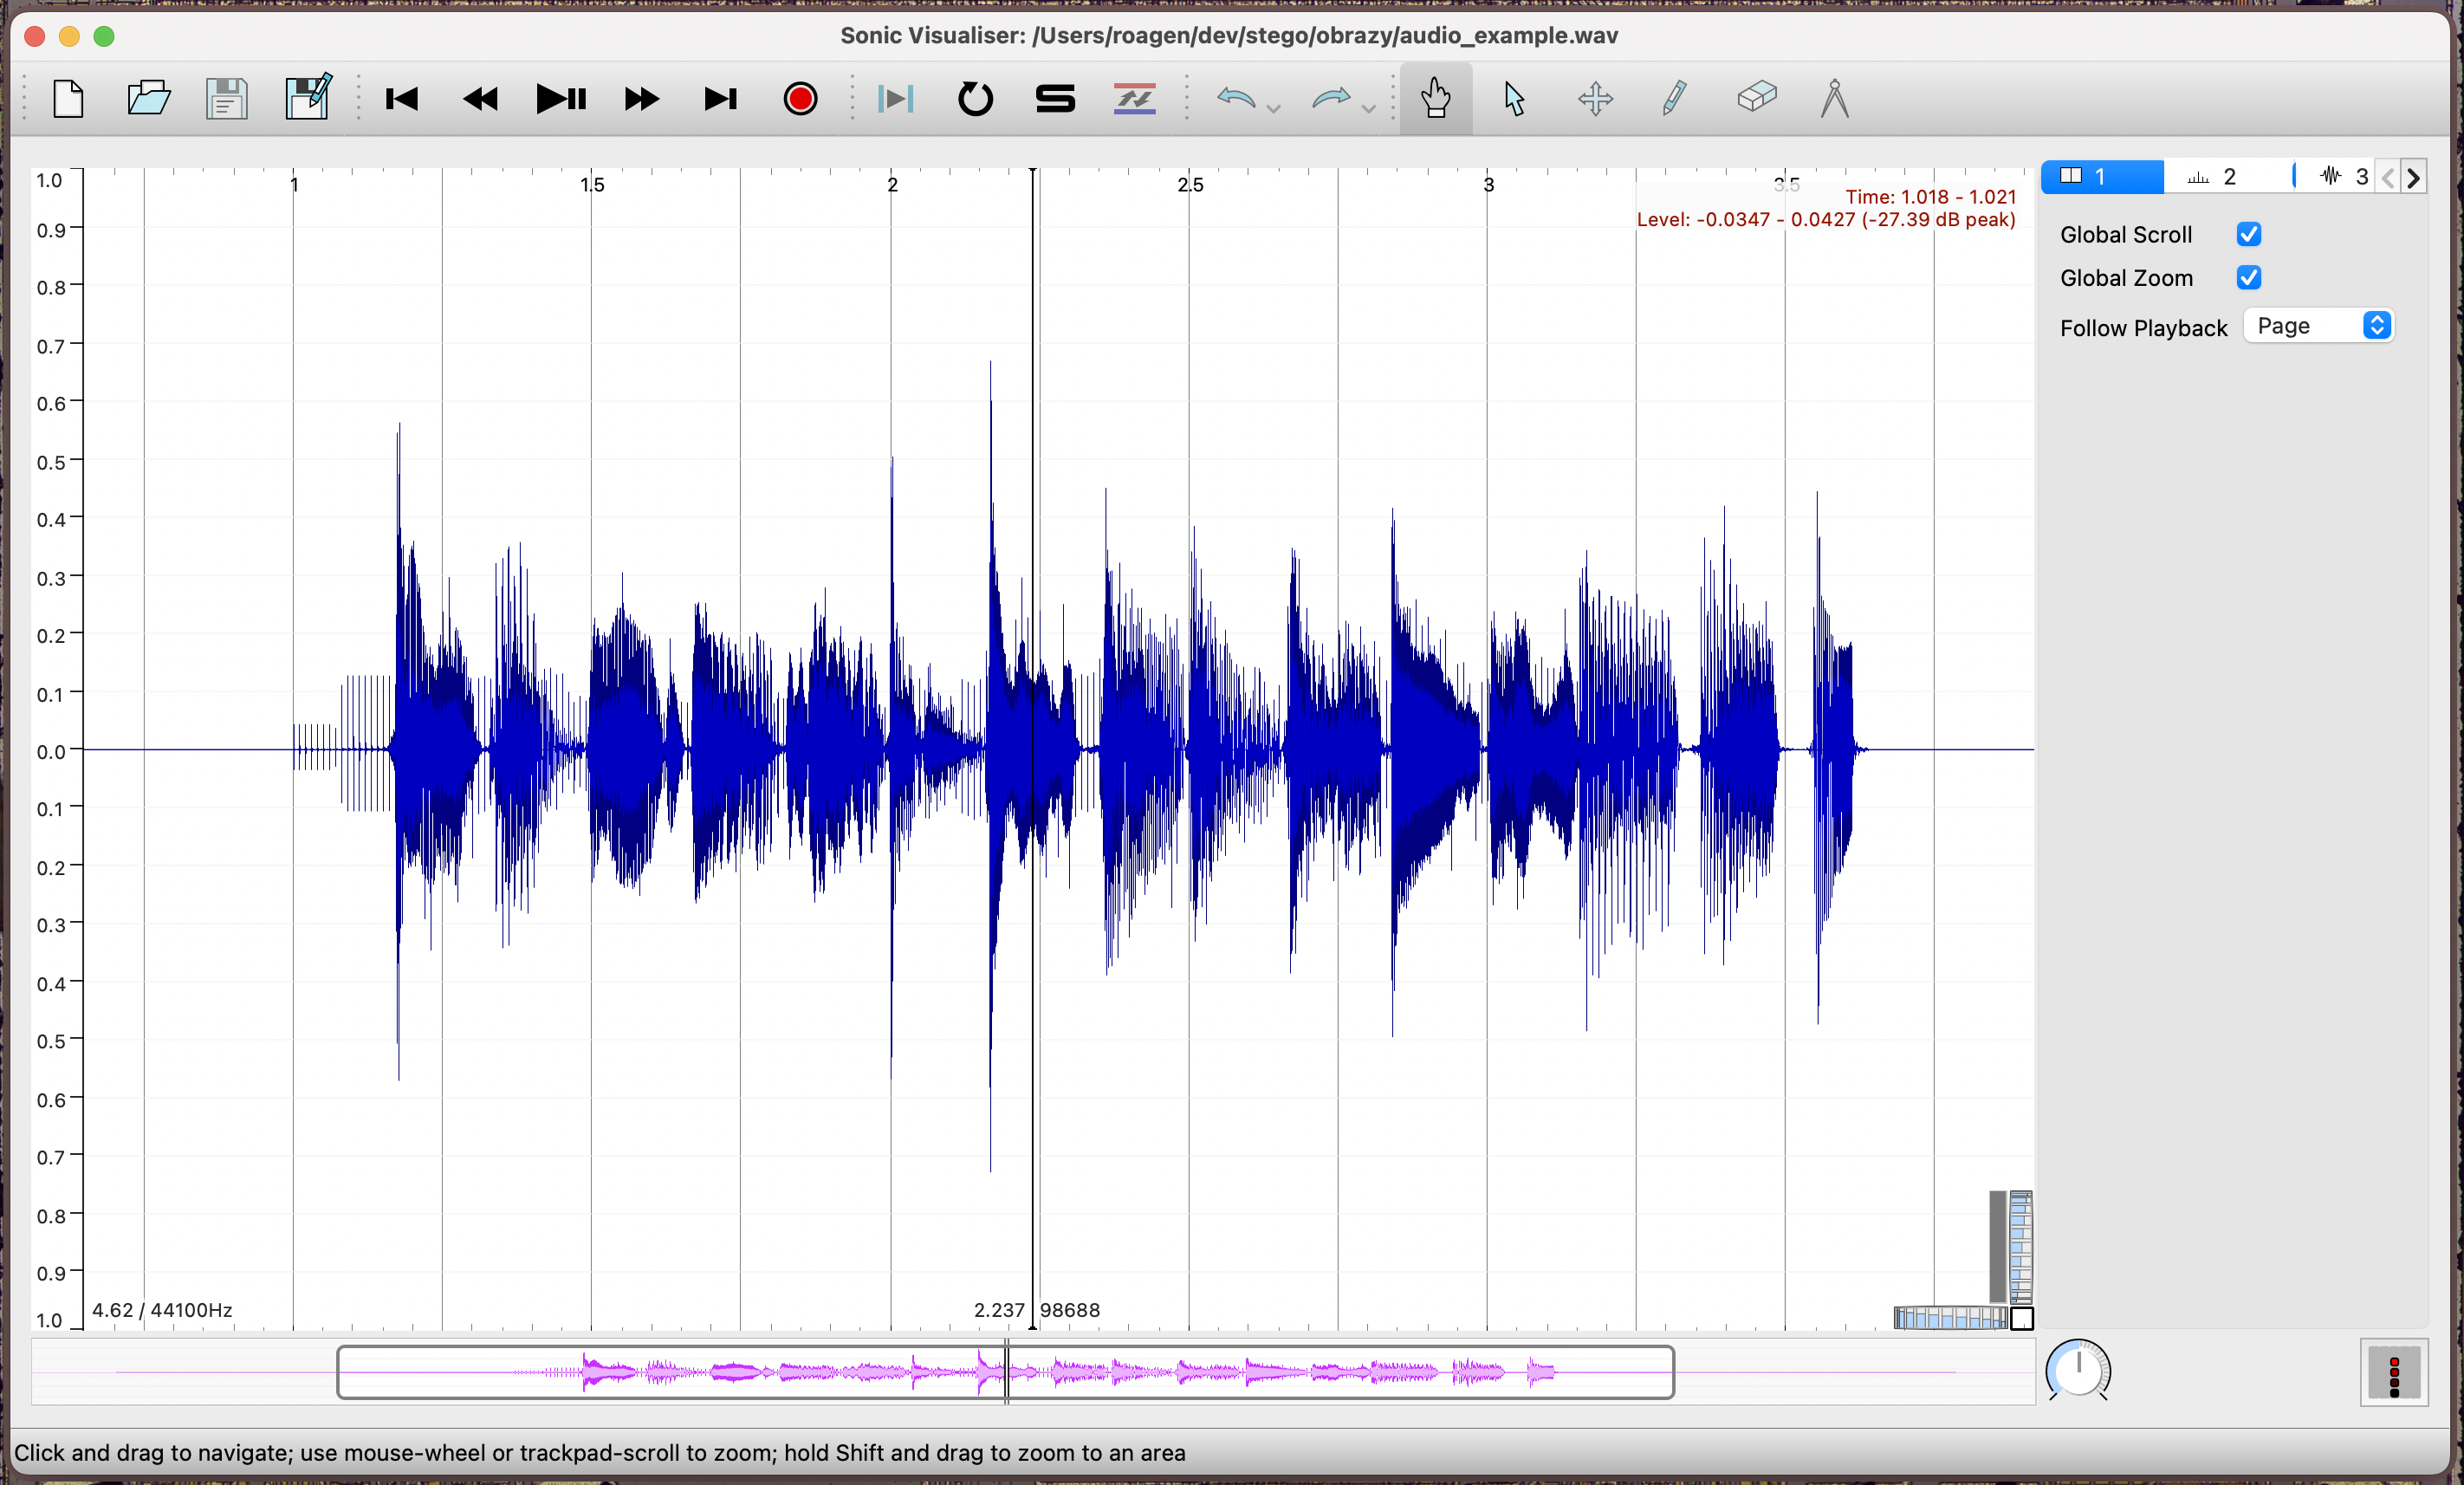
\includegraphics[width=8cm]{sonic}
	\caption{ilustracja wizualizacji sygnału z podejrzanym szumem}
\end{figure}

\section{Źródła}
\begin{itemize}
	\item \url{https://pl.wikipedia.org/wiki/Steganografia_drukarkowa}
	\item \url{https://royalprice.ru/pl/setting/steganografiya-i-stegoanaliz-obzor-sushchestvuyushchih-programm-i-algoritmov/}
	\item \url{https://www.researchgate.net/figure/The-model-of-steganography-and-steganalysis_fig1_333772050}
	\item \url{http://datagenetics.com/blog/september12015/index.html}
	\item \url{https://holloway.nz/steg/}
	\item \url{https://en.wikipedia.org/wiki/Polyglot_(computing)}
	\item \url{https://github.com/livz/cloacked-pixel}
	\item \url{https://github.com/b3dk7/StegExpose}
	\item \url{https://link.springer.com/chapter/10.1007/11424826_54}
	\item \url{https://github.com/fallais/tweg}
	\item \url{http://datagenetics.com/blog/september12015/index.html}
	\item \url{https://carlmastrangelo.com/blog/gamma-steganography}
	\item \url{https://pl.wikipedia.org/wiki/Mikrokropka}
	\item \url{https://pl.wikipedia.org/wiki/Steganografia}
	\item \url{https://en.wikipedia.org/wiki/Chaffing_and_winnowing}
	\item \url{https://www.researchgate.net/figure/Chaff-and-winnow-based-encryption_fig1_2360410}
\end{itemize}

\end{document}

